\section{Timeline}

The following section describes the project development, progress and decisions we took through the time the project was developed. After a series of informal meetings, the project officially started in February 2012 and was submitted in September 2012.

\subsection{Initial Project Meetings and Early Implementation Decisions}

The regular project meetings where we discussed mostly the organizational aspects and the top-level design of the application started in December 2011. We easily agreed that we were aiming to create an application quite similar to Google Documents. We have decided very early to use a multi-tier architecture consisting of

\begin{itemize}
\item core translation memory,
\item user space,
\item graphical user interface,
\end{itemize}

\noindent which became very soon separate Maven modules, as we soon started using Maven for building the project.

After overcoming the problems connected with learning the new technology, we became quite satisfied with the decision to use Maven, because it enables to easily combine the parts of the project.

\subsubsection{Project structure}

Despite the fact that we added further modules later, we consistently kept the initial project separation into \emph{Core}, \emph{User Space} and \emph{GUI}. At the beginning, we also assigned team members to different parts of project, which remained relatively stable as well.

\subsubsection{Initial data}

Before receiving the data from OpenSubtitles.org, we were thinking about the source of data to fill the translation memory for the first time. There were several options -- either using the subtitle part of the Czech-English parallel corpus CzEng developed at ÚFAL \footnote{\url{http://ufal.mff.cuni.cz/czeng/}}, using sentences from a general purpose parallel corpus or getting the data from a subtitles server.

\subsubsection{Programming languages}

From the very beginning, we intended to base the project on Java, mainly because there are a number of web technology projects based on Java and
 every team member was familiar with the language. 
We also decided to combine the code in Java and Scala programming 
languages. At that time, there was 
only one team member who knew the Scala language. Although we 
repetitively expressed believes that everyone of us would learn it, at 
the end there was only one other person familiar with the Scala language.

The decision to use both Java and Scala appeared to bring a number of 
complications. On one hand, Scala allows to write concise and efficient 
code; on the other hand, most project members were not able to learn 
Scala sufficiently even to understand the Scala code properly, let alone 
actively producing Scala code, and only used Java.
Although the interoperability between Scala and Java works well in most 
cases because both are based on the JVM, some problems remain. One of the 
problems of interoperability was, for example, that a \emph{List} object 
created in Scala is not compatible with Google Web Toolkit, which expects 
a standard Java \emph{List} implementation.

\subsubsection{Technology for the Client: Google Web Toolkit}
\label{subsubsec:implementation:gwt}

Much more complicated to agree on was the technology of the client. There were many different opinions, from writing the client in {\it PHP} with {\it Nette Framework}, which some of us knew well, to using the {\it JSP} to have all the code consistently in Java, even to quite an extreme idea to make the whole application a {\it Java Applet} (this idea had appeared because of the intention to integrate the video player in the application, since at that time we did not know any other way to do that except creating a Java applet). Finally, we decided to use {\it Google Web Toolkit}, which no team member had any prior knowledge of, but it promised making the communication between server and client and many other things very easy. 

More information about the decision for using GWT and a discussion of its advantages and disadvantages can be found in Section~\ref{sec:reasonsForGWT}.

%Similarly to the Scala language problem, we ended up with only three people able to work efficiently with the Google Web Toolkit. Fortunately, this did not became a bottleneck of the development process.

% I guess me (Ruda) and Honza have probably mastered GWT, but Karel is also quite fluent in it



\subsection{Early Development Process}

Luckily for us, we very soon received a database from {\it opensubtitles.org} containing all the Czech and English subtitle files that were at the server at that time. Soon after that we started working on an alignment algorithm to retrieve the parallel data from the subtitle files (the process is described in Section~\ref{sec:aligning_subtitles}) and enable us to start experiments that helped us to decide which database system could be used.


\subsubsection{Database system}

Choosing an appropriate database system was also an intensively discussed issue. The database underlying the Translation Memory plays a crucial role for the whole system performance. Also using built-in features could save us a lot of additional work.
We evaluated different DBMS and decided to use \postgres~(see Section~\ref{sec:dbms} for details). To test its applicability for our project, we ran several small evaluations of \postgres~features that might be useful to us, e.g.\ the full-text search. As soon as we made the final decision on which DBMS to use, we refactored the evaluation code into {\tt TranslationPairSearcher} classes and started to set out the general architecture of the core. The {\tt BackoffTranslationMemory} class was added and the candidate search was finished in its early stages, so a basic version of the system could be used even though there were no sophisticated rankers yet. For more details on the core architecture, please see Section~\ref{sec:corearchitecture}.

Not having any experience with the object-relation mapping libraries in Java, we decided to use {\it Hibernate}, based on advice from both Internet forums and some of our colleagues.


\subsubsection{Data alignment}

Originally, all the algorithms processing the data we retrieved were implemented in Perl, and the code for importing the data was in the \emph{Core} module, implemented in Scala. Later, to make the code more consistent, we decided to move the data preparation and data import to a separate \emph{dataimport} module and to re-implement the Perl scripts in Scala.

\begin{figure}[h]
\begin{center}
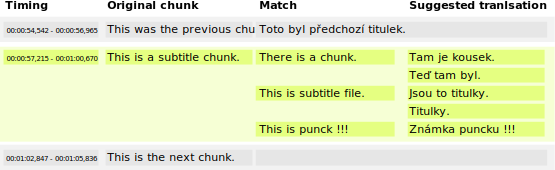
\includegraphics{./figures/original_strucutre.pdf}
\end{center}

\caption{Scheme of the originally intended structure of work with the translation memory. It reflects the original User Space structure and also schematically the original client design.}\label{fig:original_scheme}

\end{figure}

\subsubsection{Video playback}

Very soon, we started to try to solve the video playback in the browser, which we expected to be a really challenging issue. We did some research about \emph{Adobe Flash} technology. We were also thinking about creating a hybrid solution -- an application wrapper with a web browser inside, capable to ensure the video playback for the inner web application.

We very soon had toy implementations of:

\begin{itemize}
\item a player using VLC plugin, to be incorporated into the web application
\item a player as a desktop application, showing the web application in a frame (see Figure~\ref{fig:figures_desktop-app-player})
\end{itemize}

\begin{figure}[h!]
	\centering
		\includegraphics[width=7cm]{figures/desktop-app-player.png}
	\caption{Screenshot of Qt-based desktop application.}
	\label{fig:figures_desktop-app-player}
\end{figure}

We decided for the web application-only version, with no desktop variant, because, observing the development trends, it seems to us that the present and future of applications is in web applications. The benefits are e.g.\ that the learning curve is typically better for a web application, where the user is already familiar with most of the controls and work patterns, installation is not required, so anyone can start using the application immediately, it is easy to use OpenID registration.

Still, there are disadvantages, especially the cross browser support issues, limited power, and larger bandwidth consumption.
An added advantage of GWT is that the bandwidth consumption is actually closer to that of a standalone desktop app, because the application itself is stored in one JavaScript file, which is downloaded at the beginning (similar to installing a desktop application, but it is done transparently), and the rest of the client-server interaction is done through RPCs (basically the same way as it would be done in a desktop application).

An issue we encountered in developing the player and were not able to combat completely is letting the user choose a media file and passing its full file system path to the player. We found out that although it is quite easy to load a whole file from disc into memory, only its filename is passed to JavaScript instead of the full path for security reasons. We did a thorough search on the Internet but found out that there is most probably no clean way around this restriction.

Ultimately we came up with 3 solutions, but none of them pleased us enough:

\begin{itemize}
\item the user inputs the full path as a string into an input box; works well but is not user-friendly (most users probably do not even know that such a thing as a file path exists)

\item the user chooses the file in the file browser and then copies the file path from the browser input box into a textbox; this is probably even less user-friendly

\item a Java applet is loaded to choose the file as Java applets do not have such restrictions as JavaScript, and then passes the path to the application; it seems to us too heavy-weight to create and load a whole applet only to get the file path, but it works quite well -- except for the users who do not have Java installed and working properly (we have also encountered an alternative using Flash for the same purpose, but we still prefer using Java to Flash)
\end{itemize}

Despite having its disadvantages -- it is not particularly fast and from the users' view it could be considered not be really safe -- we decided for the third option.

\subsection{Introducing the Shared Classes}
\label{subsec:introducing_shared_classes}

After having implemented a very basic version of all three parts of the project, we decided it was time to start to solve the interoperability of individual parts in order to run a first snapshot of the application. This was happening approximately in March 2012.

At this stage we found out that we are not fully taking advantage of using the Java technologies for all parts of project and decided to totally redesign the User Space and Client parts.

Originally, we wanted to keep the traditional translation memory structure where each sentence can have several matches and these matches can have several translations in the memory, as is depicted in Figure~\ref{fig:original_scheme}. However, this scheme did not reflect much the way we worked with the data
in the Core, moreover there were not much cases where there would more translations for one match.

Also, the design of the GUI was a little bit confusing because the text of the matches was placed more prominently than the translation suggestions, despite the fact that the user is probably much more interested in the actual translation suggestions than in the matches. This lead to a modified scheme which is depicted in figure \ref{fig:new_scheme}.

\begin{figure}
\begin{center}
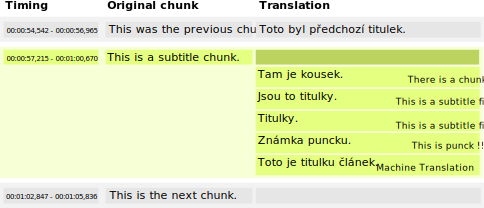
\includegraphics{./figures/current_strucutre.pdf}
\end{center}
\caption{Current scheme of the work with translation memory.}\label{fig:new_scheme}
\end{figure}

We agreed on the shared classes that all parts of the project should use. We more or less adopted the design of the classes from the core and started to use them in the whole project. This step required to re-implement some Scala classes in Java and to drop code that was already done in the User Space and the client. The design of the classes was almost the same as the final shared class design.

From a later point of view, it appears to be an important decision to agree on the shared classes, which made the cooperation between the modules easier and less verbose.


\subsubsection{GUI layout}

We started the work on the project with the new design soon, which lead to a period of struggles with technologies. It took us almost two months to have the first running version of the application.

The very first version of the application was a page where it was only possible to upload a subtitle file and to do the translation, without any possibility to load an already saved subtitle document or download the result of the translation, without any sessions or users; it was just a page where you edit the subtitles (which later became the Translation Workspace).


\subsubsection{External APIs}

At that time we used machine translation from the MyMemory service (which in fact wraps Google Translate), but there is a limited access per IP address and we soon began to reach the limit very frequently. It became obvious the we would have to change the source of machine translation. Based on that we decided to train our own Moses system. See Chapter~\ref{chap:moses} for details.

We also used an API providing IMDB.com information to receive information 
about movies but the movie meta data was not used in the evaluation the 
matches at that time. We had to switch to Freebase later because the IMDB service we used was discontinued.

\subsection{The Main Development Phase}

It is hard to define the main development phase which is covered in the 
following paragraphs. It corresponds to the period from the beginning of 
March when the important design changes were made (see previous 
Section~\ref{subsec:introducing_shared_classes}) to approximately the 
middle of August when adding new features was stopped (see the next 
Section~\ref{subsec:final_development}).

The section is divided to parts covering the issues we were dealing with 
and describes what we did in each area in those approximately five and 
half months.

\subsubsection{OpenID}
\label{subsubsec:openid}

Although we wanted to implement OpenID support from the very beginning, 
we started with it approximately in May. We found the two most frequently 
used Java libraries for OpenID and tried them. Those were \emph{JOpenID} 
and \emph{openid4java}.

\emph{JOpenID} seemed to be easier to use and also was much smaller as a 
dependency; on the other hand, when we ran into some problems with using 
it, we found out that \emph{openid4java} is much more frequently 
discussed on the \emph{StackOverflow.com} forum and that there is a 
bigger chance that we would be able to find some advice for potential 
problems. 

However, as discussed in \ref{us:openid}, \emph{openid4java} is easier to implement, so we used that, even for its biggest shortcoming -- users are not able to set their own OpenID provider.

The support for OpenID was finished in July, the parser for the authentication data from Seznam was added at the beginning of August.

\subsubsection{Chunk Splitting}

An interesting issue, also from the linguistic view, we had to solve was to find the best way of splitting the subtitle items into chunks. As opposed to the classical way of simply splitting documents into sentences, we had several possible ways of doing the splitting because of the nature of subtitle files.

We talk about chunk splitting more in chapter~\ref{os:sentence_splitting}.

We then realized that it is important that the splitting the same when importing subtitles into the database and when processing the user subtitles (as discussed in~\ref{os:guiparsing}), so we made it a shared class.

\subsubsection{Logging GUI}

After a while we found out that logging GUI errors is as important as logging userspace and core errors. We describe the GUI logging in section~\ref{gui:logging}; we first had a temporary debugging console, we switched it to remote logging mechanism at the beginning of August.

\subsubsection{Implementing the RPCs}

From the start, it was obvious to us that we want to use a well-established method to implement the Remote Procedure Calls.
We noted in the specification that we would probably use JSON for the message serialization.
Fortunately, GWT does provide a ready-to-use Remote Service implementation, which is described in bigger detail in chapter~\ref{sec:rpc:rpc}. GWT,  as a matter of fact, does actually serialize the messages to JSON internally.


\subsubsection{Sending Translation Results}

What we have been almost continually changing was the way the results are requested and then sent back by User Space. The discussion is described in greater detail in Section~\ref{sec:rpc:discussion_sending_results}.

\subsubsection{User Management}

At the very beginning the GUI was basically only the translation workspace. It was possible to translate a subtitle file in the application, the changes were reflected in the database, however it was not possible to get them in the application when the web application was reloaded or to export the subtitles.

We considered the user management to be just a minor technical issue. However, to enable to reach the intended architecture of the User Space -- mostly that most of the calls should be resolved in the Session objects -- we introduced a simple fake login in April (you could log as any user using password "guest").

We started to implement the OpenID login support in May (see Section~\ref{subsubsec:openid}). When we met some technical difficulties, we decided to implement our own registration and login first.

For more information about user management, see part \ref{us:usermanag}.

\subsubsection{GUI Look and Feel}

The design of the GUI was driven by the intentions of effectiveness, while retaining a smooth look at the same time. The effectiveness was achieved by stressing the keyboard-oriented control of the components and simplicity of their layout. The need of a pleasant visual feeling was the reason for using the Twitter Bootstrap design, bringing a user friendly feeling of the application at a very little cost.

\begin{figure}
\begin{center}
\includegraphics[scale=0.5]{figures/old_screenshot.png}
\end{center}
\caption{Design of the Translation Workspace before starting to use the Twitter Bootstrap}
\label{fig:before_bootstrap}
\end{figure}

\subsubsection{GUI Pages}

We started having one page only, the Translation Workspace, which was sufficient for development of the application for several months. Later we added the Document  Creator page as the default one, which replaced itself by the Translation Workspace once a document was created, and this was sufficient for some more time. However, we eventually could not avoid adding more pages and the need to explicitly handle multiple pages became obvious.

This lead to some problems, because GWT cannot easily handle more pages, which genuinely surprised us.

We describe the problems and their solutions in the chapter~\ref{gui:gwt}


\subsubsection{Handling Parsing Errors}

% At first, the subtitle files were expected to be in the correct format -- no explicit checks were performed and if an error was encountered, the file was rejected.
% The SrtTime class was then added 

We found that since many subtitle files are partly or fully generated by users, and probably also because the SRT format has no official specification, errors in the files are very common. Rejecting even the files with only minor errors (such as a surplus or missing newline, or an incorrect time format which we check thoroughly) showed to be unnecessarily strict, as typically most of the file is correct and the number of errors is small.

We decided to introduce heuristics to decide whether to reject the whole file: if the number of recoverable errors is lower than 10, the erroneous parts are skipped and the rest of the file is parsed.


% However, this lead to also rejecting
% We were improving the situation gradually, eventually creating a new exception class, InvalidDocumentFormatException, which is thrown by the parser, with a 
% Also, as a preliminary check, we refuse any file which is larger than 500 kB. We introduced this check because it is very fast and efficient.

\subsubsection{Offline Mode}
\label{ip:subsubsec:offline}

At first, our intention was to make the whole application able to run offline. However, it was not a priority and was not even part of the official specification.

When we tried the HTML5 Local Storage, though, the offline mode seemed to be actually easy to implement using this technology, while the support for it is good across web browsers.

The Offline mode is described in bigger detail in Chapter~\ref{gui:offlinemode}


\subsubsection{Subgestboxes}

One of the most important features of the application's user interface is the behavior of the actual translation workspace, particularly the text-boxes where user writes their translations and which provide the pop-up suggestions from the translation memory. Since the functional requirements for these boxes were gradually refined throughout the development process, their implementation also underwent several stages of evolution. However, their class\' name, {\tt SubgestBox}, remained from the early stages, implying the idea of a box offering suggestions for subtitles.

Since the GWT pre-implemented {\tt SuggestBox} did not meet our requirements we had to find our own solution using HTML IFrames and GWT {\tt RichTextArea}. It provided all the functionality we have requested, but there was a significant performance problem -- the browser often became irresponsive when loading hundreds of them. We solved this by distinguishing so-called ``fake'' and ``real'' {\tt SubgestBoxes}; it is described in bigger detail in Chapter~\ref{gui:subgest}.


%We don't want to repeat GUI chapter
%The {\tt RichTextArea}, being based on the IFrame HTML element, provided all the functionality we have requested (although some of it is not as simply accessible as we expected), but there was yet another problem with it. Having one IFrame for each chunk on the page, i.e. hundreds of them for an average movie, turned out to be quite a significant performance problem -- the browser often became irresponsive. In the end, we have solved this issue by distinguishing so-called ``fake'' and ``real'' {\tt SubgestBoxes}; the former being simple {\tt TextAreas} and displayed by default in the translation workspace, on focus transforming into the latter, the real IFrame-based {\tt SubgestBoxes} with all the functionality. This also required special approach in CSS styling.

Another issues as focus handling, automatic scrolling, dealing with endlines (see Table~\ref{implprocess:RichTextAreaNewlines} for details) and automatic resizing had to be solved in order to make the Translation Workspace more user-friendly.

\begin{table}[h]
\smaller
\begin{center}
\begin{tabular}{|l|l|l|}
\hline
\textbf{Browser} & \textbf{getText()}             & \textbf{getHTML()} \\
\hline
Firefox & \verb=first linesecond line= & \verb=first line<br>second line<br><br>= \\
\hline
Chrome  & \verb=first line=            & \verb=<div>first line</div><div>second line</div><div><br></div>= \\
        & \verb=second line=           & \\ 
\hline
Safari  & \verb=first line=            & \verb=first line<div>second line</div><div><br></div>= \\
        & \verb=second line=           & \\
\hline
IE9     & \verb=first line=            & \verb=<p>first line</p><p>second line</p><p>&nbsp;</p>= \\
        & \verb=second line=           & \\
\hline
Opera   & \verb=first linesecond line= & \verb=<p>first line</p><p>second= line</p><p><br></p> \\
\hline
\end{tabular}
\end{center}
\caption{Table capturing different handling of newlines across browsers, showing the return values of the RichTextArea's getText() and getHTML() methods. In all the cases, the text entered was ``first line[enter pressed]second line[enter pressed]''.}\label{implprocess:RichTextAreaNewlines}
\end{table}

\subsubsection{Subtitles Export}

When implementing the subtitles export feature, we encountered an unexpected issue:
GWT cannot create a new file, neither on server (because it is all JavaScript) nor on the user's computer (because of security restrictions).

We found several possible solutions:

\begin{itemize}

\item export the subtitles into a text area
\begin{itemize}
\item the easiest to implement
\item not what a user expects
\item not easy to use for the user
\end{itemize}

\item send the exported subtitles to user's e-mail address
\begin{itemize}
\item quite easy to implement because we already have implemented the e-mail sending
\item might be useful for some users
\item not what a user expects
\item can be hard to use for the user
\item might be added as a special feature but should not be the only or primary way
\end{itemize}

\item create a temporary file on the server and offer a download link to the user
\begin{itemize}
\item expected behavior from the user (file download using the browser)
\item reasonably reliable
\item reasonably easy to implement
\item should handle access rights in Jetty which is an added complication
\item creating temporary files is not very clean
\end{itemize}

\item create a new servlet (using JSP) for downloading the file
\begin{itemize}
\item expected behavior from the user (file download using the browser)
\item probably the cleanest possible solution
\item we were afraid that it would be too much extra work, but we realized that it was not so difficult
\end{itemize}

\end{itemize}

Eventually, we decided for the last option as the best one; therefore, the User Space actually consists of two servlets, one to handle RPCs and another for file download.

\subsubsection{Chunks saving/loading}

We originally decided that the subtitle file will be parsed in the GUI, 
to avoid unnecessary sending of the data from GUI to User Space and then back from User Space to GUI; parsing the file in User Space would also cause unnecessary load on the server.

Although we wanted to make everything as parallel as possible, we found out that we have to save all the chunks immediately after parsing so that they do not get lost; therefore, requesting the translation suggestions is only done after that, even though this means that the translation suggestions start arriving a little later.

To also enable editing the files, the Translation Workspace became the only page that has two constructors -- one receiving the text of a subtitle file to parse, and the other getting an already parsed document from the database.

\subsubsection{Finalizing and training the translation pair rankers}

Although the candidate search was started early in the development process, the ranking of candidates was not completed until the main development phase. Since we base the ranking on combining various scores with weights, it is necessary to estimate these weights from data. In order to produce the annotated data for this, all other parts of the system had to be fully functional. Because of this, we could finalize the ranking and train the ranking models only later in the main development phase.

\subsubsection{Machine translation}
Altough machine translation with Moses was thought to be just a nice possibility to have and weren't given too much attention initially, at the end we were very surprised with how accurate it is on our data (seeing it being more successful than Google Translate was a \emph{very} gratifying moment) and how quick we managed to finally get it.

The only problematic part was fitting both our application and Moses on the same small virtual machine we were given for this project. However, when we deleted all unnecessary data from the disk and ran with only the binarized models, we were able to run it fine (even when we have only about 1 GB of free disk space, but it seems to be enough for Jetty).

\subsection{Final Development}
\label{subsec:final_development}

We left many issues which we considered to be only minor and technical
to the end of the development process;
some of these issues were eventually found to constitute intensive work.

We set the Feature Freeze to the 12$^\mathrm{th}$ August, 12 p.m.
After the Feature Freeze, no new features were added to the project, and 
we started an intensive review of already existing code, debugging, and 
working on the documentation. After the feature freeze, we improved 
stability of the application and its responsiveness. 


\section{Evaluating the Development Process}

\subsection{Technologies}
One of the crucial decision for the project was the choice of technologies. Most of the technologies we used -- Maven, Scala, Hibernate, GWT -- were new to some of us and we also had not much experience with the other. Combining these technologies together was a difficult task and would probably even be for an experienced Java developer. Generally, because we were not too very familiar with the technologies, we spent most of the time solving technical issues. There are numerous research challenges, mostly in the fuzzy matching part, which had to remain untouched due to that. Nevertheless, it is doubtful if this was caused only by technical difficulty or by paying too much attention to less important technical tasks.


A bottleneck of the development process was also that not all of us were familiar with all of the technologies. It happened several times that somebody could not continue developing a particular part of the project and had to wait for another team member to fix the issue.

On the other hand, our choice of technologies appeared to also be good since it saved a significant amount of work for us due to the possibility to share an implementation of a class. Using the Scala language for the core also made the parallelization much easier.

\subsection{Structure}
Although we spent a long time on discussions of how the structure of the project would look like, we did not avoid a radical change of the design of the application a few months after the project started. Nearly the whole User Space code had to be dropped and it was also necessary to totally remake the client components existing so far.

\subsection{Efficiency, communication}
During the whole time we had the problem that our development process was not as effective as we would imagine and it was also difficult to find a suitable communication platform. Although we saw each other often to discuss the project issues and had regular meetings, a working online communication played a crucial role for us.

As a very first communication channel, we established a mailing list at Google groups. All the notifications and comments from Github were redirected to that mailing list, as well as results of Jenkins builds. Soon, we started to receive dozens of FilmTit email every day and it started to be quite difficult the follow the conversations and find items in the conversation history.

Because of this, we tried to use PiratenPad\footnote{\url{http://www.piratenpad.de/}}. It is free a web-based collaborative real-time editor, allowing authors to simultaneously edit a text document, and see all of the participants\' edits in real-time, with the ability to display each author's text in their own color. There is also a chat box in the sidebar to allow meta communication. The service is run by the German Pirate Party. We tried to use the tool to gather personal plans and ``todos'', bug reports, etc. After some time, the pads became messy and the mailing group became the main communication channel again. We were also solving many issues bilaterally using various instant messaging systems.

In July, %when the most intensive work on project started,
we launched a Skype group chat. It effectively replaced the personal meetings, which was much sought after as usually several members were out of Prague at a time, but fortunately, they typically had an Internet connection.
It also helped to solve many issues instantly and efficiently.
However, it has a same disadvantage as email conversation -- it is difficult to easily find facts in the history -- but now with hundreds of messages every day to make things worse.
Fortunately, because almost every time there were at least some team members online, it was always possible to ask for a summary of the previous discussions and we managed to keep all the team members informed about everything important.

%Mid-August, however, there was a decline in using the Skype group -- we found out that when all of the project members were online and the work on the project could have been expected to be very intensive, it often actually happened that very little work was done since most of the time was spent on discussions through Skype.
%Another issue was that some members tended to use the conference simply for chatting about non-related matters, %including me of course --R
%which later made it even harder or nearly impossible for the others to find important messages in the history.
%We then started to send the most important messages through the e-mail conference again and, eventually, we mostly switched back to it.


\section{Work Distribution}

\subsection*{Karel Bílek}

\begin{itemize}
	\item implementation of the VLC playback and java applet
	\item processing the OpenSubtitles.org data
	\item preparing and optimization of the Moses system to our use
	\item initialization of Jetty webserver
\end{itemize}

\subsection*{Josef Čech}

\begin{itemize}
	\item development of the User Space
\end{itemize}

\subsection*{Joachim Daiber}

\begin{itemize}
	\item design and implementation of the Core Translation Memory, searching, ranking, merging, import, indexing, media source retrieval, etc.
	\item evaluation of database systems
	\item parts of the GUI layout, stylesheet and general fixes in GUI
	\item set up continuous build system, initial Maven project, configuration management
\end{itemize}



\subsection*{Jindřich Libovický}

\begin{itemize}
	\item early processing of the opensubtitles.org data
	\item design and implementation of the User Space
\end{itemize}


\subsection*{Rudolf Rosa}

\begin{itemize}
	\item development of many functions of GUI (login, Offline Mode, pages, dialogs, settings etc.)
	\item Remote Procedure Calls and their GUI implementation
\end{itemize}


\subsection*{Jan Václ}

\begin{itemize}
	\item development of the GUI (structure, visual appearance and experience, Translation Workspace)
\end{itemize}


\section{Possible Future Development}

There are many issues to be improved, mostly in the graphical interface. It would probably be possible to add new features forever. A newer version would likely include support for more language pairs.

We would like to let the project run for some time and wait if it would find its community of users. If it would reach some success among the user, it could provide much interesting data -- mostly about preferences of the users about which translation suggestions are useful for them. Such information could be useful for developing new fuzzy matching techniques including some research challenges, such as finding matches to only a part of a sentence. Success among users would also mean a growing source of well structured data for statistical machine translation.

